Each test needs to join together results obtained from different databases.

This operation is not trivial, since a query cannot be directly performed across multiple databases.

The solution I opted for was creating a script on Databricks, from which each database can be queried independently, the results can be put together and additional operations can be performed.

\subsection{Why Databricks?}
   The test suite has been developed on Databricks for several reasons.
    
    \paragraph{Already accessible}
        First of all, this environment was already accessible, since it has been used for the ETL process.
        Using an existing environment requires little to no additional configuration, and its costs are already included in the project budget.
    
    \paragraph{Multiple languages}
        Secondly, Databricks supports multiple languages in the same workbook.
        The query results have been merged using Python, while additional analyses have been performed on the resulting dataset in SQL, taking full advantage of the strengths of both language.
    
    \paragraph{Spark}
        A third important aspect is that Databricks natively supports Spark, meaning that each database could be queried at the same time.
        Moreover, each query is automatically parallelized to further improve their performance.
    
\subsection{Script Description}
    \begin{figure}
        \centering
        \begin{subfigure}{\textwidth}
            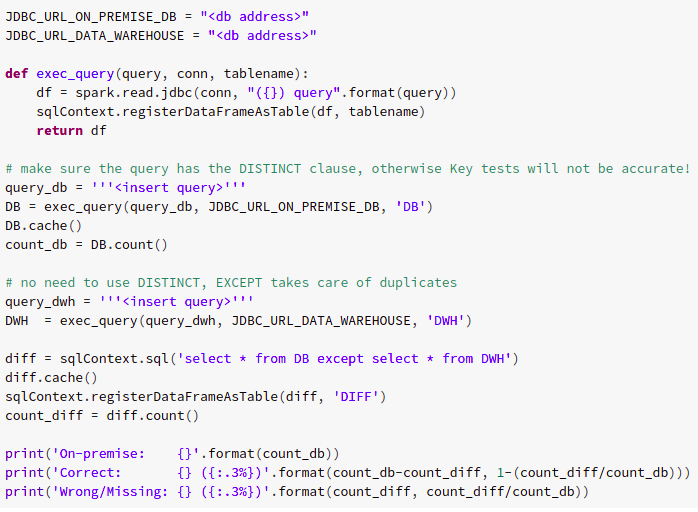
\includegraphics[width=\textwidth]{res/tests/test_suite.png}
            \subcaption{Python}
        \end{subfigure}
        
        \begin{subfigure}{.3\textwidth}
            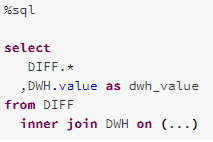
\includegraphics[width=\textwidth]{res/tests/test_suite_sql.png}
            \subcaption{SQL}
            \label{fig:tests:data:suite:sql}
        \end{subfigure}
        
        \caption{Testing suite.}
        \label{fig:tests:data:suite}
    \end{figure}

    The script created, shown in Figure \ref{fig:tests:data:suite}, requires as input two queries.
    
    The first query will be performed on the on-premise database, while the second on the Data Warehouse.
    These queries must return data in the same format, since the results are going to be merged.
    
    By using Spark, the scripts performs a join between both results, taking all values from the on-premise database which have not been found in the Data Warehouse.
    
    From this new dataset it is possible to compute the data match percentage between the two databases.
    
    \paragraph{SQL}
        A separate cell, using SQL, allows users to perform \textit{ad-hoc} queries on the mismatching values, which has been used abundantly to analyze the problems found.
        
        For example, the query shown in \ref{fig:tests:data:suite:sql} compares the values stored in each database, excluding the rows which are present only in the local database.
        This query proved to be extremely useful for understanding issues related to Value tests.